\lecture{Sept. 28}


\begin{thm}
Assume that $\{a_n\}$ converges. then $\{a_n\}$  is bounded.
\end{thm}

\begin{proof}
Assume that $$L = \lim_{n\to \infty} a_n$$
Let $\epsilon = 1$. Then there exists $N_0 \in \mathbb{N}$ so that if $n\geq N_0$ then $|a_n-L|<1$

If $n\geq N_0$,then \begin{align*}
    |a_n|=|a_n-L+L| &\leq |a_n-l|+|L|\\
    & < 1+|L|
\end{align*}

Let $$M = max {|a_1|,|a_2|,\dots ,|a_{N_0-1}|,|L|+1}$$.

Then $|a_n|\leq M$ for all $n\in \mathbb{N}$.
\end{proof}

\textbf{Question: }Do all bounded sequences converge? \hfill No.

\begin{defn}
\begin{enumerate}
    \item We say that a sequence $\{a_n\}$ is increasing if $a_n<a_\{n+1\}$ for all $n\in \mathbb{N}$
    \item We say that $\{a_n\}$ is non-decreasing if $a_n\leq a_{n+1}$ for all $n\in \mathbb{N}$
    \item We say that $\{a_n\}$ is decreasing if $a_{n+1} <a_n$ for all $n\in \mathbb{N}$
    \item We say that $\{a_n\}$ is non-increasing if $a_{n+1} \leq a_n$ for all $n\in \mathbb{N}$
\end{enumerate}

We say that $\{a_n\}$ is monotonic if $\{a_n\}$ satisfies one of the conditions.
\end{defn}

\textbf{Example: }
\begin{enumerate}
\item
$$\{a_n\} = \{\frac{1}{n}\}$$
is decreasing, since $$\frac{1}{n+1}\leq \frac{1}{n}$$ for all $n\in \mathbb{N}$
\item $$\{cos(n)\}$$
\item Let $a_1=1$,$$a_{n+1} = \sqrt{3+2a_n}$$


\begin{figure}[ht]
\centering
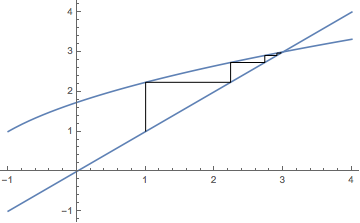
\includegraphics[width=0.6\textwidth]{picture/1.png}
\caption{$y=\sqrt{3+2x}$ and $y=x$}
\end{figure}
%image

\end{enumerate}

\begin{thm}\textbf{Monotone Convergence Theorem}

If $\{a_n\}$ is monotonic and bounded, then $\{a_n\}$ converges.
\end{thm}

\begin{proof}
Assume that $\{a_n\}$ is non-decreasing and bounded above. Let $L = lub(\{a_n\})$

Let $\epsilon > 0$, then $L-\epsilon$ is not an upper bound. Then there exists $N_0\in \mathbb{N}$ so that $L-\epsilon < a_{N_0} \leq L$. If $n\geq N_0$, then $L-\epsilon < a_{N_0} \leq a_n \leq L$, so $|a_n - L| < \epsilon$. Hence $L = \lim_{n\to \infty} a_n$

Similarly, if $\{a_n\}$ is non-increasing then $L = \lim_{n\to \infty} a_n$ where $L = glb(\{a_n\})$
\end{proof}

\begin{exmp}
Let $a_1=1$,$$a_{n+1} = \sqrt{3+2a_n}$$
\end{exmp}

We know that $0\leq a_n < a_{n+1} \leq 3$ for all $n\in \mathbb{N}$. $\{a_n\}$ is increasing and bounded above. Hence $\{a_n\}$ converges.


\begin{cor}
A monotonic sequence $\{a_n\}$ converges iff it is bounded.
\end{cor}

\begin{defn}
We say a sequence \textbf{diverges to $\infty$} if for every $M>0$ we can find a a cutoff $N_0 \in \mathbb{N}$ such that if $n\geq N_0$, then $M\leq a_n$, we write $\lim_{n\to \infty} a_n = \infty$.
\end{defn}


